\let\negmedspace\undefined
\let\negthickspace\undefined
\documentclass[journal]{IEEEtran}
\usepackage[a5paper, margin=10mm, onecolumn]{geometry}
\usepackage{lmodern} 
\usepackage{tfrupee} 
\setlength{\headheight}{1cm}
\setlength{\headsep}{0mm}   

\usepackage{gvv-book}
\usepackage{gvv}
\usepackage{cite}
\usepackage{amsmath,amssymb,amsfonts,amsthm}
\usepackage{algorithmic}
\usepackage{graphicx}
\usepackage{textcomp}
\usepackage{xcolor}
\usepackage{txfonts}
\usepackage{listings}
\usepackage{enumitem}
\usepackage{mathtools}
\usepackage{gensymb}
\usepackage{comment}
\usepackage[breaklinks=true]{hyperref}
\usepackage{tkz-euclide} 
\usepackage{listings}                             
\def\inputGnumericTable{}                                 
\usepackage[latin1]{inputenc}                                
\usepackage{color}                                            
\usepackage{array}                                            
\usepackage{longtable}                                       
\usepackage{calc}                                             
\usepackage{multirow}                                         
\usepackage{hhline}                                           
\usepackage{ifthen}                                           
\usepackage{lscape}
\usepackage{xparse}

\bibliographystyle{IEEEtran}

\title{4.7.59}
\author{EE25BTECH11062 - Vivek K Kumar}

\begin{document}
\maketitle

\renewcommand{\thefigure}{\theenumi}
\renewcommand{\thetable}{\theenumi}

\numberwithin{equation}{enumi}
\numberwithin{figure}{enumi} 

\textbf{Question}:\\
Find the equation of a line perpendicular to the line $x + 2y + 3 = 0$ and passing
through the point $\brak{1, -2}$.

\textbf{Solution: }

\begin{table}[H]    
  \centering
  \begin{tabular}{|c|c|}
\hline
\textbf{Name} & \textbf{Value} \\ \hline
$\vec{A}$ & $\myvec{2 & 1 \\0 & 3}$ \\ \hline
\end{tabular}

  \caption{Variables used}
  \label{tab:4.7.59}
\end{table}

The given line can be expressed as 
\begin{align}
    \vec{n_1}^\top \vec{x} = c \\
    \myvec{1 & 2}\vec{x} = -3\\
\end{align}

As the given lines are perpendicular
\begin{align}
    \vec{n_1}^\top \vec{n_2} = 0 \\
    k = \frac{-1}{2}\\
    \vec{n_2} = \myvec{1 \\ -1/2}
\end{align}

The equation of the resulting line can be expressed as
\begin{align}
    \vec{n_2}^\top\brak{\vec{x} - \vec{A}} = 0\\
    \myvec{1 & \frac{-1}{2}}\vec{x} = \myvec{1 & \frac{-1}{2}}\myvec{1 \\ -2}\\
    \myvec{1 & \frac{-1}{2}}\vec{x} = 2
\end{align}

\begin{figure}[H]
   \centering
  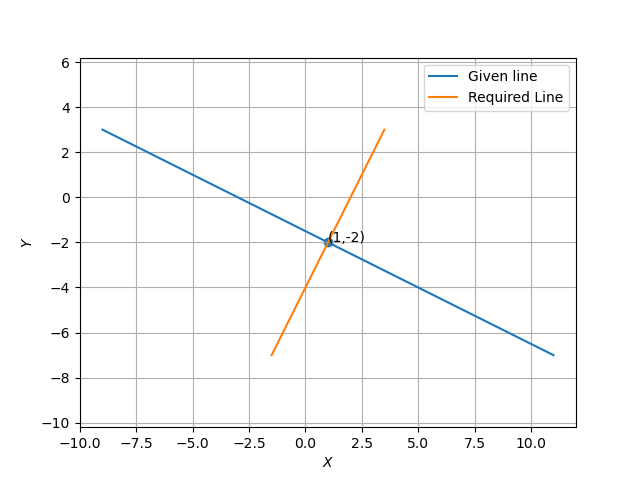
\includegraphics[width=0.64\columnwidth]{figs/fig.png}
   \caption{Given points on a line}
   \label{stemplot}
\end{figure}
\end{document}  
